\zotelo{../thesis.bib}

\chapter{Introduction}
\label{chap:intro}

Neutron stars are compact stellar objects made of degenerate nuclear matter with radius $\sim 10$~km.
They are fascinating objects in both observational and theoretical astrophysics as well as fundamental physics.
Observationally, neutron stars have exhibited extremely stable radio pulsations, X-ray and $\gamma$-ray emissions. 
Past and current observations including Integral, RXTE, 
Chandra, 
XMM-Newton, 
NuSTAR, 
Swift, 
and Fermi
have revealed to us various transient and persistent radiative activities from the radio band to $\gamma$ ray band.
Moreover, the LIGO detection of GW170817 for the double neutron star merger event \citep{2017ApJ...848L..12A} has enabled the first multi-messenger astrophysical observation with gravitational waves.
On the theory side, to understand the high energy radiation from neutron stars poses an important problem for theoretical astrophysics.
This task involves deep knowledge of basic physical processes in the extreme astrophysical environment including hydrodynamics and magnetohydrodynamics, radiative processes, acceleration of nonthermal particles and magnetic reconnection.
Besides, the structure and cooling of neutron stars requires input from nuclear physics for the many body physics under the strong interactions and neutrino physics.
Moreover, the strong gravity near the neutron star makes it an ideal place to test the general relativity under strong gravity.

A particular type of neutron stars, named magnetars, is observed to show soft $\gamma$-ray bursts with very short rise time ($\lesssim 1$~ms) and luminosity up to $10^{47}$~erg/s, much larger than their spin-down power.
Unlike normal neutron stars whose radiations are powered by the rotational energy, it is believed that radiative events of magnetars are powered by the release of magnetic energy of an ultra-strong magnetic field $10^{14}-10^{16}$~G. 
The presence of strong magnetic fields brings more interesting physics relevant to magnetars.
Crustal materials of magnetars behave differently under the strong magnetic, and they show new mechanical and thermal properties. 
In particular, the nuclear lattice in the magnetar crust can be broken by the strong magnetic stress and become plastic.
Magnetic energy released from the crustal failures must be transported from the interior of the magnetar to the magnetosphere and dissipate there to power observed emissions.
This process involves the coupled dynamics of magnetic fields inside and outside the magnetars as well as the magnetohydrodynamics in a relativistic magnetic dominated plasma which is still not fully understood.

This dissertation will be focusing on several problems of electrodynamics of magnetic fields from the interior to the magnetosphere. 
In this section, we will give brief review of relevant background knowledge of neutron stars, magnetohydrodynamics as well as magnetars. An outline of this thesis will be given at the end of this section.
Throughout this dissertation, the notation $X_m$ stands for the quantity $X$ normalized to $10^m$ in the cgs unit.

\section{Neutrons Stars}
\label{sec:intro-NS}

\subsection{Theoretical and observational discovery}

Soon after the discovery of neutrons \citep{1932Natur.129Q.312C} in 1930s, \citet{1934PhRv...46...76B} envisioned the existence of neutron stars as the final products of supernova explosions.
Meanwhile, \citet{1935MNRAS..95..226C} during his research of the final phase of stellar evolution, proposed the idea of white dwarfs -- a star supported by the quantum effects of electron degenerate pressure that acts against gravity.
However, the white dwarfs can only sustain a maximum mass of around $1.4M_\odot$ which is the so-called Chandrasekhar mass limit and heavier stellar object with residual mass larger than the mass limit will continue their gravitational collapse.
As the stars keeps collapsing, it is more favorable for electrons to combine with protons through the inverse $\beta$-decay to form neutrons.
When the stellar density reaches the neutron drip density $\sim 4\times 10^{11}$~g/cm$^3$, the neutron degeneracy pressure becomes the main effect that counteracts the gravitationally collapse.
Such compact stellar objects that can be formed through the balance between neutron degeneracy pressure and gravity collapse are neutron stars.
Due to their high density, general relativistic effect must be considered for neutron stars. \citet{1939PhRv...55..364T} and \citet{1939PhRv...55..374O} derived the equation of neutron star structure from the hydrostatic equilibrium in general relativity in a spherical symmetric setting
%
\begin{equation}\label{eq:TOV}
	\frac{d P}{dr} = -\frac{G M}{r^2} \rho \left(1+\frac{P}{\rho c^2} \right) \left( 1+\frac{4\pi r^3 P}{M c^2} \right) \left( 1-\frac{2GM}{rc^2} \right)^{-1}
\end{equation}
%
where $r$ is the radial coordinates, $\rho$ is the density of the degenerate matter, $P$ is the pressure and $M$ is the total mass enclosed within radius $r$.
The above TOV equation should be supplemented with the equation of state, an equation that determines the pressure as a function of density to fully solve the structure of the neutron stars.

Until 1960s, neutron star has remained a pure theoretical idea which was employed by theorists to explain the X-ray sources in the sky \citep{1964Natur.201.1308M} . 
In 1967, a very regular radio pulses was discovered by \citet{1969Natur.224..472H} at the Mullard Radio Astronomy Observatory.
This radio source has a period of $1.337$~s at the frequency of $81.5$~MHz at extreme accuracy. 
The extreme constancy of the frequency suggests was then soon associated this object with a rotating neutron star \citep{1968Natur.218..731G} where strong magnetic fields and high rotational speed of the star accelerate the surrounding plasmas and lead to a beacon-like radiation pattern.
The name pulsar was coined for such neutron stars with pulsating radio emissions powered by their rotations.
%
\begin{figure}[h]
  \centering
  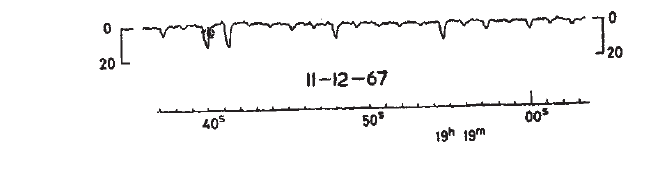
\includegraphics[width=0.8\textwidth]{pics/intro/pulses.png}
  \caption[A record of pulsating radio source]{A record of the pulsating radio
    source discovered in 1967 \citep{1969Natur.224..472H}}
  \label{fig:pulse}
\end{figure}
%

As more pulsars were discovered, slowing down of pulsar rotations were also discovered that enabled the estimation of spin-down luminosity from their angular velocity $\Omega$ and angular acceleration $\dot{\Omega}$ or the period $P$ and its derivative $\dot{P}$
%
\begin{equation}\label{eq:spin_down}
	  L_{d} = -I\Omega\dot{\Omega} = 4\pi^2 I\frac{\dot{P}}{P^3}
\end{equation}
%
where $I$ is the moment of inertia of the pulsar.
For the Crab pulsar with period $P=33$~ms and $\dot{P}=4.2\times 10^{-13}$ \citep{1968IAUC.2113....1L}, its spin-down luminosity is $10^{39}$~erg/s which agreed with the observed luminosity.

Our current knowledge attributes the spin-down of the pulsars to their magnetic field. For the simplest case, the pulsar magnetic can be modeled as a magnetic dipole with strength $\mu$.
As the giant magnetic dipole of pulsar is rotating, it is radiating away its rotational energy at the luminosity
%
\begin{equation}\label{eq:dipole_rad}
	L_{d} = \frac{2}{3}\frac{\mu^2\Omega^4}{c^3}.
\end{equation}
%
Equating Equation~\ref{eq:spin_down}  and Equation~\ref{eq:dipole_rad} can lead to an estimation of magnetic field at the surface of the neutron star
%
\begin{equation}
		B_0 = 3.2\times 10^{19}\sqrt{P \dot{P}}\,\mathrm{G}.
\end{equation}
%
For normal pulsars parameters, the resulting surface magnetic fields are of order $10^{12}$~G.
Such high magnetic fields also eliminate the possibility that radio pulsars being white dwarfs and establish rotating neutron stars as the standard theoretical explanation of pulsars.

Apart from radio emission, neutron stars are also visible in X-ray and $\gamma$-ray bands. Several neutron stars including the Crab \citep{1974Natur.251..397K} and Vela \citep{1975ApJ...200L..79T} were discovered to have pulsed $\gamma$-ray emissions at the period as the radio pulses. 
Geminga pulsar, on the other hand, was a radio-quiet $\gamma$-ray source with soft X-ray pulses \citep{1992Natur.357..222H} suggesting the $\gamma$-ray and radio emissions origin from different regions.
The {\it Fermi} satellite discovered over 130 $\gamma$-ray pulsars \citep{2010ApJS..188..405A}.
These $\gamma$-ray pulsars can be classified into three groups: millisecond pulsars, young radio-loud pulsars and young radio-quiet sources.
 Many neutron stars are also X-ray sources. Their X-ray radiation is usually made up of two components: a thermal component from the surface cooling and a non-thermal component from the magnetospheric emission \citep{2006csxs.book..279K}.
 
 \subsection{Structure of neutron stars}
 \label{sec:intro-structure}
 
The structure of a non-rotating unmagnetized neutron star is governed by Equation~\ref{eq:TOV} together with the equations of state.
The equation of state must be determined from the underlying physics that describes the interaction of the neutron-rich nuclear matter.
Depending on the density, the structure of a neutron star can be divided into two regions: the core and the crust. 
The core of a neutron star refers to the region where $\rho>\rho_{\rm nuc}$ with $\rho_{\rm nuc}=2.8\times 10^{14}$g/cm$^3$ being the density of nuclear saturation which accounts for $\sim 99\%$ of the total mass of the star.
The outer layer where $\rho<\rho_{\rm nuc}$ is the neutron star crust.
%
\begin{figure}[h]
  \centering
  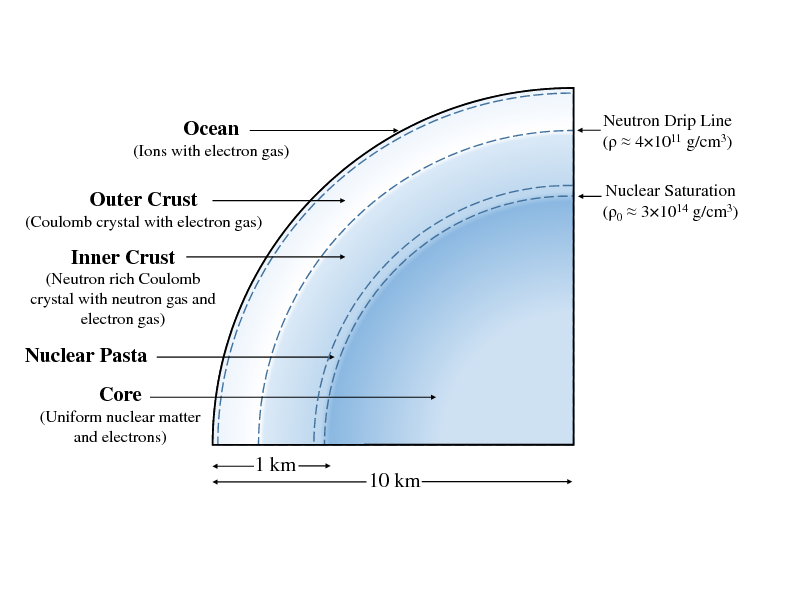
\includegraphics[width=0.8\textwidth]{pics/intro/NS_structure.png}
  \caption[A cartoon illustrates the structure of a neutron star] {A cartoon illustrates the structure of a neutron star \citep{2017RvMP...89d1002C}}
  \label{fig:NS-structure}
\end{figure}
%
\subsubsection{Core}
The neutron star core is composed of a mixture of neutrons, protons and electrons and possibly muons.
All constituents are highly degenerate and interact through nuclear force to form a strongly non-ideal liquid.
Calculation for the equation of state and the composition of highly degenerate nuclear matter from nuclear physics is very uncertain especially at high density $\rho>2\rho_{\rm nuc}$.
Exotic forms of matter like hyperionic matter ($\Sigma^-$ and $\Lambda$ hyperons), pion condensate, kaon condensate and quark matter might exist at such a high density.  
\citet{1959NucPh..13..655M} predicted that neutron in neutron stars can become superfluid.
The neutron gas can form superfluid through the singlet-state ($^1 S_0$) Cooper paring [see \citet{2003RvMP...75..607D} for a review].
The critical temperature $T_{\rm crit}$ below which the crustal neutrons become superfluid is sensitive to uncertainties in modeling many-body strong interactions. The characteristic value is $T_{\rm crit} \lesssim 10^{10}$~K [e.g. \citet{1999PhyU...42..737Y,2001LNP...578...30L}], with significant uncertainties \citep{2004ARA&A..42..169Y, 2009ApJ...707.1131P,2012MNRAS.422.2632H,2015PhRvC..91a5806H}.

%
\begin{figure}[h]
  \centering
  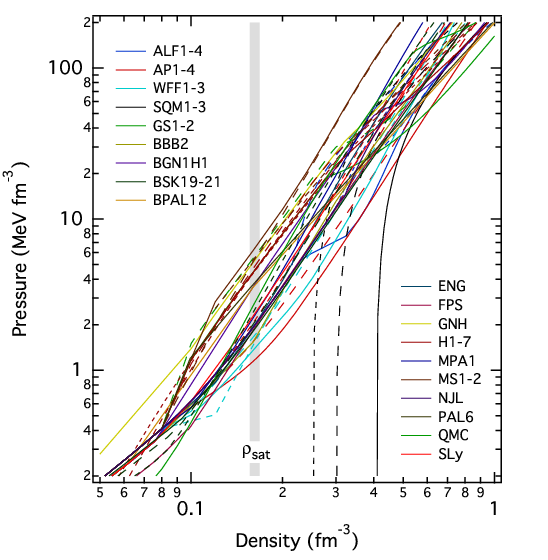
\includegraphics[height=0.4\textwidth]{pics/intro/eos.png}
  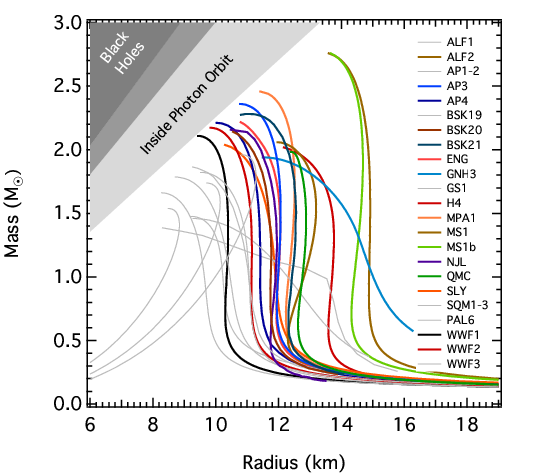
\includegraphics[height=0.4\textwidth]{pics/intro/mass-radius.png}
  \caption[Equation of state and mass-radius relation for neutron stars] {{\it Left:} Pressure as a function of density for various theoretical models. {\it Right:} Mass-radius relation for various neutron star equation of state \citep{2016ARA&A..54..401O}}
  \label{fig:NS-eos}
\end{figure}
%

The left panel of Figure~\ref{fig:NS-eos} shows different neutron star equations of state from various theoretical models and the right panel shows the resulting mass-radius relation from the corresponding equation of state.
Observational constraints of the neutron star equation of state mainly come from the measurements of mass and radius of neutron stars.
The determination of J1614-2230 to have mass $2M_\odot$ \citep{2010Natur.467.1081D} can eliminate all theoretical models with maximum mass smaller than it.

Neutrino emission is also generated through various channels in the neutron star and affects the cooling of neutron stars and the emissivity is very sensitive to the temperature $T$.
In the center of the core, Direct urca cooling (hereafter Durca) is the fastest neutrino emission mechanism
%
\begin{equation}
	   \dot{q}_\nu^D\sim 10^{27}\,T_9^6\, \mathcal{R}_D {\rm~erg~s}^{-1}{\rm cm}^{-3} \:\:\: (\rho\gtrsim 10^{15} {\rm~g~cm}^{-3}),
\end{equation}
%
where $\mathcal{R}_D\leq 1$ is a suppression factor that appears in the presence of 
superfluidity \citep{2001PhR...354....1Y}.  
However, it is activated only if the separation between the Fermi levels of protons and neutrons is sufficiently small, which occurs
at $\rho\gtrsim 10^{15}$~g~cm$^{-3}$.
Such high densities are only found in neutron stars with masses  $M \gtrsim 1.4 M_\odot$ \citep{1991PhRvL..66.2701L}.

Neutron stars with masses $M\lesssim 1.4M_\odot$ do not activate Durca, and the cooling occurs with a lower rate due to the modified urca reactions (hereafter Murca), which involve a spectator nucleon taking the excess momentum.
Murca occurs everywhere in the core with the cooling rate given by 
(\citealp{1979ApJ...232..541F}),
%
\begin{equation}
	\label{eq:Murca}
  \dot{q}_{\nu}^M\sim  7\times 10^{20}
  \,T_9^8 \left(\frac{\rho}{\rho_{\rm nuc}}\right)^{2/3} \mathcal{R}_M
    {\rm ~erg~s}^{-1}{\rm ~cm}^{-3},
\end{equation}
%
where $\rho_{\rm nuc}=2.8\times 10^{14}$~g~cm$^{-3}$ is the nuclear saturation density.
With the onset of proton or neutron superfluidity the Murca rate is suppressed by the 
factor $\mathcal{R}_M<1$, and the main cooling process becomes``Cooper pair cooling'' ---  
neutrino emission that accompanies the formation and breaking of Cooper 
pairs \citep{1976ApJ...205..541F,2009ApJ...707.1131P}. Its rate is given by
%
\begin{equation}
   \dot{q}_\nu^{CP}\sim 10^{21} \left(\frac{\rho}{\rho_{\rm nuc}}\right)^{1/3} T_9^7 
    \; f\left(\frac{T_{\rm core}}{T_{\rm crit}}\right) {\rm ~erg~s}^{-1}{\rm ~cm}^{-3}, 
\end{equation}
%
where the numerical factor $f(T_{\rm core}/T_{\rm crit})$ describes the temperature dependence of the Cooper pair cooling; $f=0$ at $T_{\rm core}>T_{\rm crit}$, $f$ steeply reaches a maximum at $T_{\rm core}\approx 0.8 T_{\rm crit}$ and steeply declines at $T_{\rm core}<0.5 T_{\rm crit}$.
%
\begin{figure}[h]
  \centering
  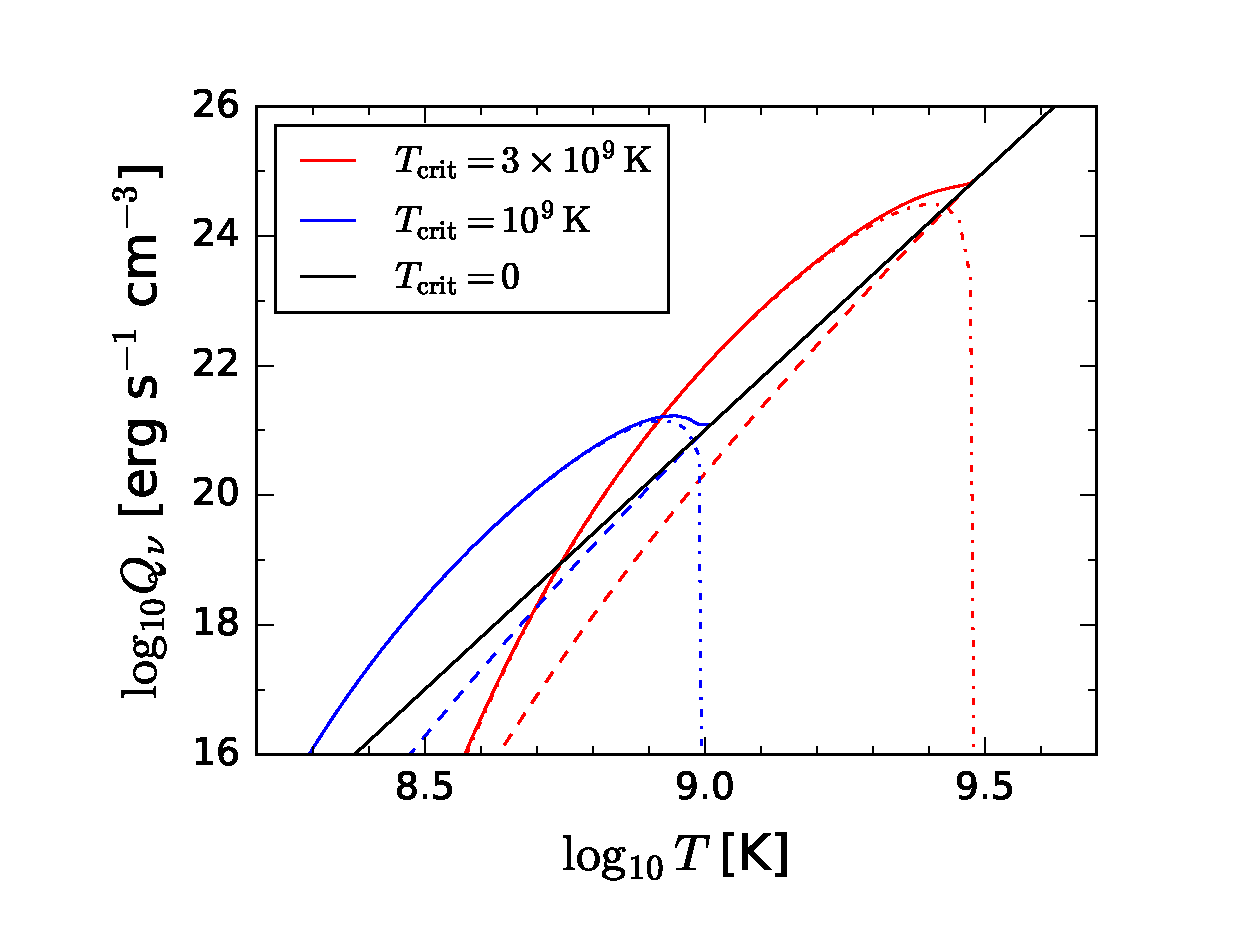
\includegraphics[height=0.6\textwidth]{pics/intro/qv.eps}
  \caption[Neutrino cooling rate in the core of neutron stars] {Neutrino cooling rate as a function of temperature in the core matter at density $\rho_{\rm nuc}=2.8\times 10^{14}$~g~cm$^{-3}$. Black curve shows Murca cooling assuming no superfluidity ($T_{\rm crit}<10^8$~K). Colored curves show the cooling of matter with non-superfluid protons and superfluid neutrons, for two cases: $T_{\rm crit}=10^9$~K (blue curves) and $T_{\rm crit}=3\times 10^9$~K (red curves). Dashed curve shows the Murca contribution and dash-dotted curve shows the Cooper pair contribution; the net cooling rate is shown by the solid curve.
The triplet-state neutron pairing is assumed (model B in \citealp{2001PhR...354....1Y})}
  \label{fig:NS-qv}
\end{figure}
%

\subsubsection{Crust}

The neutron star crust is elastic solid composed of Coulomb lattice of nuclei with degenerate electrons and neutrons.
The degenerate electrons are ultra-relativistic and the electron capture process $e^-+p\rightarrow n + \nu_e$ becomes more effective with increasing density which makes the matter more neutron-rich.
In the outer crust where density is lower than the neutron drip density $\rho_0=4\times 10^{11}$~g/cm$^3$, the pressure is dominated by the degenerate electron gas.
In the inner crust $\rho>\rho_0$,  neutrons start to drip out of the nuclei and form a free fermionic gas. Heavy nuclei, degenerate electrons, degenerate neutrons and free neutrons coexist and the pressure is dominated by the free neutrons.
Close to the core-crust interface, nuclei are more energetically favorable to have anisotropic shapes \citep{1983NuPhA.407..571R}. 
These new phases of nuclear matter are named as nuclear pasta phases. They are the transitive states to the uniform nuclear matter in the core and can have observational signature on the transport properties of neutron stars  \citep{2017RvMP...89d1002C}. 
The outermost $\sim 100$~m of the crust, called envelope or ocean, is low-density ($\rho<10^9$~g/cm$^3$) liquid.
Their chemical composition can be heavy nuclear like iron or light element if the neutron star accretes matter from its companion in a binary system.

Even though the crust only accounts for a small fraction of the mass of the neutron star, it is crucial for many astrophysical phenomena of the neutron stars.
The core of the neutron has high thermal conductivity and remain isothermal, and it is the thermal properties of the crust that govern the heat transport rate and therefore the surface temperature of the neutron star.
The specific heat of the crust are dominated by degenerate electrons and ions \citep{2015SSRv..191..239P}. Neutrons also contribute to the specific heat above the neutron drip point, however, their contributions will be greatly reduced once neutrons become superfluid.
The thermal conductivity is governed by the degenerate electron gas and increases with density. A static temperature profile in the crust will exhibit a constant temperature in most part of the crust with a sharp temperature gradient sustained in the envelope that governs the surface temperature of the neutron star.   
With the presence of strong magnetic fields, it is more energetically favorable for the degenerate electrons to stay in the lowest Landau level. 
Especially, when the energy of the lowest Landau level $\hbar e B/m_e c$ is larger than the rest mass energy $m_e c^2$ (i.e. $B>B_{\rm QED}\equiv m_e^2 c^3/\hbar e=4.4\times 10^{13}$~G), all electrons are confined in the lowest Landau level.
Therefore, thermal conductivity is enhanced in the direction parallel to the magnetic fields and reduced in the perpendicular direction \citep{1996A&A...306..999P,1996A&A...314..341P}.

Neutrino emissions in the crust become efficient cooling mechanism once internal or external heating increase the temperature above $10^9$~K. 
The main channels for neutrino emission in the crust are plasmon decay, electron-nucleus bremsstrahlung, electron-positron annihilation and electron synchrotron radiation if strong magnetic fields are present \citep{2001PhR...354....1Y}.

\section{Magnetars}
\label{sec:intro-magnetars}

% TODO: Introduce magnetars, and open up the historical observation discussions
Magnetars are a class of neutron stars with ultra-strong magnetic fields. 
They exhibit giant flares, bursts and outbursts in the band of hard X-ray to soft $\gamma$-rays. 
Unlike normal pulsars which are powered by the rotational energy, magnetar activities typically have radiation luminosity much larger than their spin-down power.
The ultimate energy source of their violent radiative activities is the strong magnetic field inside and outside the neutron stars.

\subsection{Discovery}
\label{sec:intro-magnetar-discovery}

In 1979, the interplanetary probes Venera 11 and 12 reported repeated bursts in the band of hard X-ray and soft $\gamma$-ray \citep{1979SvAL....5...87M}.
At first, these events were first classified as classical Gamma Ray Bursts (GRBs), but the repeated bursts in the star-forming Dorado region in the Large Magellanic Cloud including a giant flare \citep{1979Natur.282..587M} suggested they were a new class of high energy radiative events. 
The bursts exhibited strong evidence that they came from neutron stars.
They had very short rise time $\sim 15$~ms, implying the a relativistic motion over the distance of the size of a neutron star.
A $8$~s pulsating period was also observed in the tail of the light curve is consistent with the rotational period of a neutron star, though much slower than other young neutron stars like the $33$~ms Crab pulsar.
As more repeated bursts were subsequently discovered including SGR 1806-20 \citep{1987ApJ...322L..21K,1987ApJ...320L.111L} which showed around $100$ bursts between 1978 and 1986, these sources were finally recognized as a new class of high energy radiative events, Soft Gamma Ray Repeaters (SGRs).

Meanwhile, another mysterious class of objects, Anomalous X-ray Pulsars (AXPs) were also discovered whose strong X-ray luminosity exceeded the spin-down power.
The first object was discovered in the supernova remnant CTB 109 using the Einstein observatory \citep{1980Natur.287..805G}, with a spin period of $3.5$~s \citep{1981Natur.293..202F}.
Later, two other sources were discovered, 1E 1048.1-5937 \citep{1986ApJ...305..814S} and 4U 0142+61 \citep{1994MNRAS.267..490H,1994ApJ...433L..25I}. They all showed unusually soft X-ray spectra, making AXPs a new class of objects.

\citet{1995MNRAS.275..255T,1996ApJ...473..322T} suggested that SGRs are actually neutron stars with ultra-strong magnetic fields $10^{14}-10^{15}$~G, the magnetars.
In their model, repeated bursts are powered by the decay of magnetic energy from the ultra-strong magnetic field.
\alfven waves launched from the interior of the magnetar dissipate their energy in the magnetosphere creating an optically thick pair plasma fireball that gives rise to the soft-ray emission.
\citet{1996ApJ...473..322T} also suggested that AXPs are also magnetars and should exhibit repeated bursts.

In 1998, the first SGR spin-down rate was measured for SGR 1806-20 \citep{1998Natur.393..235K}, reporting a surface dipole magnetic field $8\times 10^{14}$~G. The same measurement for SGR 1900+14 were followed shortly \citep{1999ApJ...510L.115K} with magnetic field $2-8\times 10^{14}$~G.
The identification of SGRs as magnetars were confirmed by the two measurements.
SGR-like bursts were also discovered for AXPs later \citep{2002Natur.419..142G,2003ApJ...596L..71K}, and bursts are known to be a characteristic property of AXPs.
Eventually, the astrophysical community accepted magnetars as the standard explanation for SGRs and AXPs.

Up to now, there are 29 magnetars discovered, including 15 SGRs and 14 AXPs [cf. McGill Online Magnetar Catalog at http://www.physics.mcgill.ca/~pulsar/magnetar/main.html \citep{2014ApJS..212....6O}].
Figure~\ref{fig:ppdot} shows the relation between period $P$ and its time derivative $\dot{P}$ for various pulsars and magnetars.
Due to their high dipole magnetic fields, magnetars have higher spin-down rate and larger periods, and they all sit on the top-right corner of the figure.
%
\begin{figure}[h]
  \centering
  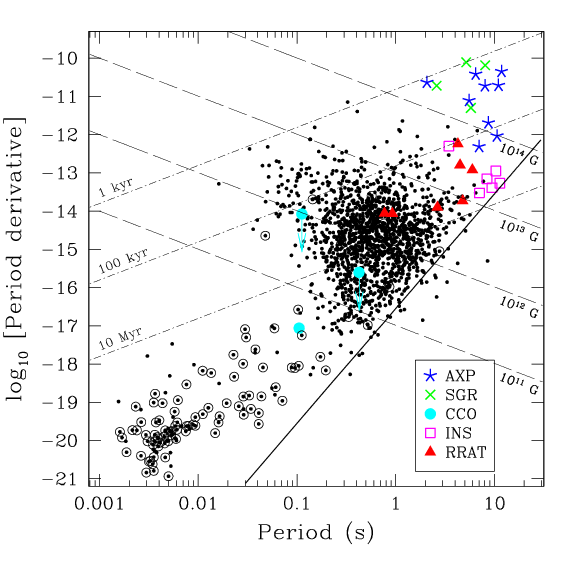
\includegraphics[width=0.6\textwidth]{pics/intro/ppdot.png}
  \caption[$P-\dot{P}$ diagram for pulsars and magnetars]{$P-\dot{P}$ diagram for pulsars and magnetars \citep{2010PNAS..107.7147K}.}
  \label{fig:ppdot}
\end{figure}
%
\subsection{Magnetar Activities}
\label{sec:magnetar-activities}

Magnetars exhibit both transient and persistent high energy radiations in forms of hard X-ray and soft $\gamma$-ray.
The transient events including soft $\gamma$-ray bursts, giant flares and outbursts.
The term burst refers to short millisecond events and giant flare refer to those violent bursts releasing energy higher than $10^44$~erg.
Outburst, on the other hand, refer to longer events with an exponential decaying afterglow on the timescale of months to years.

\subsubsection{Bursts}
Soft $\gamma$-ray bursts are the the most common transient events for magnetars. Both SGRs and AXPs exhibit bursts with a full spectrum of burst rate.
Some extremely active sources like SGR 0526-66 can become inactive for the subsequent decades \citep{2003ApJ...585..948K,2009MNRAS.399L..74T} while some quiet source like 1E 2259+586 can suddenly enter an active phase with hundreds of bursts  \citep{2003ApJ...588L..93K}.

The bursts have peak luminosity ranging $10^{36}$ to $10^{43}$~erg/s and sharp rise time from millisecond to second, with a log normal distribution peaking near $100$~ms.
The repeated bursts have power-law distribution, positive correlation between waiting times of successive events, log-normal waiting time distribution and no correlation between waiting times and intensities \citep{1996Natur.382..518C}.

\subsubsection{Giant Flares}
Giant flares are the most catastrophic radiative events of magnetars. 
There have been three events recorded up to now, all come from different sources: SGR 0526-66 on March 5, 1979 \citep{1980ApJ...237L...7E}, SGR 1900+14 on August 27, 1998 \citep{1999Natur.397...41H} and SGR 1806-20 on December 27, 2004 \citep{2005Natur.434.1098H,2005ApJ...624L.105M,2007ApJ...661..458B}.
The peak luminosity of giant flares range from $10^{44}$ to $10^{47}$~erg/s.
Figure~\ref{fig:gf-light-curve} shows the light curve for the 2004 giant flare SGR 1806-20. 
The light curve consists of two parts: an initial spike $\sim 0.2$~s followed by a long decaying tail lasting for $\sim 400$~s modulated by the rotational period of $7.56$~s.
Most energy (over $10^{46}$~erg) is released during the initial peak while the tail only radiates $10^{44}$~erg of energy.
%
\begin{figure}[h]
  \centering
  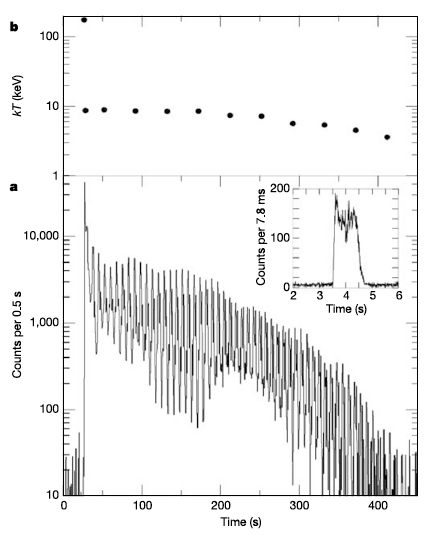
\includegraphics[width=0.5\textwidth]{pics/intro/gf.png}
  \caption[Light curve for the 2004 giant flare SGR 1806-20]{Light curve for the 2004 giant flare SGR 1806-20 \citep{2005Natur.434.1098H}.}
  \label{fig:gf-light-curve}
\end{figure}
%

\subsubsection{Outbursts}

Magnetar outbursts are characterized a sudden increase of X-ray luminosity up to $10^{36}$~erg/s, 10-1000 times of the quiescent level of radiations \citep{2004ApJ...609L..21I,2004ApJ...605..368G,2008A&ARv..15..225M,2011ASSP...21..247R}.
The outbursts are generally associated with radiative and timing anomalies such as spectral hardening, change in pulsed fraction and pulse profiles, multiple short X-ray bursts and glitches.
The light curves of outbursts usually show a long exponential decay following the bursts on the time scale of months to years. 
Figure~\ref{fig:outburst-light-curve} plots the light curves for eight different outbursts.
%
\begin{figure}[h]
  \centering
  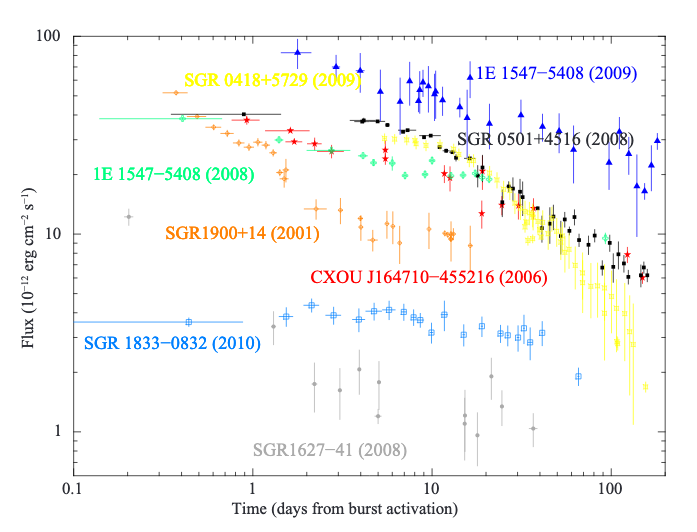
\includegraphics[width=0.6\textwidth]{pics/intro/outbursts.png}
  \caption[Light curves of eight magnetar outbursts]{Light curves of eight magnetar outbursts \citep{2011ASSP...21..247R}.}
  \label{fig:outburst-light-curve}
\end{figure}
%

Some magnetars have very low quiescent luminosities $<10^{33}$~erg/s and are discovered only when their X-ray luminosity increases by a factor of $100-1000$ during the outburst.
These magnetars are named as transient magnetars, and the first transient magnetar was discovered is XTE J1810-197 \citep{2004ApJ...609L..21I} whose flux decayed on the time scale of a year \citep{2007Ap&SS.308...79G}.

\subsubsection{Persistent emissions}

In the quiescent phase, magnetars can be divided into two different classes: the persistent magnetars and the transient magnetars.
The persistent magnetars like 1E 2259+586 or 4U 0142+61 have high quiescent luminosity $>10^{33}$~erg/s while the transient magnetars like XTE J1810-197 or SGR J1745-2900  have low quiescent luminosity.
The X-ray spectra of transient magnetars can be well modeled by a single blackbody component with temperature $k_B T\sim 0.15-0.3$~keV while persistent magnetars usually show a power-law component in addition to the blackbody component with $k_B T\sim 0.3-0.5$~keV \citep{2014ApJS..212....6O}.
The surface luminosity of persistent magnetars show a narrow range around $10^{35}$~erg/s \citep{2006ApJ...650.1070D} corresponding to the surface temperature of $0.3-0.5$~keV consistent with their X-ray spectra.
For a thousand-year-old neutron star usually have core temperature $T_{\rm core}\sim 10^8$~K and surface temperature $T_{\rm surf}\sim 10^6$~K \citep{2004ARA&A..42..169Y}, corresponding to the thermal luminosity of $10^{33}$~erg/s.
The surface temperatures of persistent magnetars are significantly higher than the surface temperature of normal neutron stars.
It is proposed that the high temperatures are sustained by the magnetic energy stored in the magnetars \citep{1992ApJ...392L...9D,1992AcA....42..145P} .

\subsection{Theoretical Models}
\subsubsection{Internal dynamics and crustal failures}
A young magnetar can have a strong toroidal magnetic component as a result of magnetohydrodynamical relaxation after its birth \citep{2009MNRAS.397..763B}.
Since the interior of a neutron star is a perfect, magnetic fields are frozen into the electron fluid and magnetic fields can move mainly through the drift of electrons with respect to the neutrons and ions.
Therefore the evolution of magnetic fields is slow in the magnetar, and main through the two process: ambipolar diffusion and Hall drift \citep{1992ApJ...395..250G}.

Ambipolar diffusion results from the motion of electron-proton plasma through the neutron fluid. 
Due to the difference of proton and electron mass, protons feel the frictional force from the collision with neutrons while electrons almost move freely.
In the core, the ambipolar diffusion  develops on the timescale $t_{\rm amb}\sim 10^3 (T_9/k_{-5}B_{16})^2$ \citep{2016ApJ...833..261B} where $T$ is the core temperature and the wave number $k\sim 10^{-5}$~cm$^{-1}$ characterizes the length scale of magnetic field variation $\pi/k$.
Pressure gradient is generated by the ambipolar diffusion but will be erased by weak interactions $e+p\rightarrow n$ \citep{1992ApJ...395..250G,2016ApJ...833..261B}.
The ambipolar diffusion tends to dissipate magnetic energy and heat up the magnetar, and the process stalls as the core temperature stalls.

Hall drift is a result of electron motion relative to ions with the velocity $\boldsymbol{v}_H = -\boldsymbol{j}/en_e$ where $\boldsymbol{j}$ is the current and $n_e\sim 10^{37}$~cm$^{-3}$ is the electron number density.
Even though Hall drift conserves energy, it can cascade energy to smaller scales and dissipate the energy through the Ohmic dissipation \citep{1992ApJ...395..250G}.
Numerical simulations of Hall evolutions in the neutron star in 2D and 3D have been studied by \citep{2009A&A...496..207P, 2016PNAS..113.3944G,2018MNRAS.473.2771B}.

Magnetar crust, like the neutron star crust, is made up of nuclear Coulomb lattices.
The magnetar crust is incompressible and immune to cracks and slips due to the huge hydrostatic pressure \citep{2003ApJ...595..342J} and magnetic fields \citep{2012MNRAS.427.1574L}.
However, the Coulomb lattice can yield to shear stresses and give rise to plastic failures.
Molecular dynamics simulations by \citet{2009PhRvL.102s1102H} and \citet{2010MNRAS.407L..54C} that plastic failures are triggered when the elastic strain exceeds the critical value $s_{\rm cr}\approx 0.1$ as shown in Figure~\ref{fig:plastic-md}.
Shear magnetic stress can be generated and accumulated in the crust through the ambipolar diffusion and the Hall drift \citep{1996ApJ...473..322T,2011ApJ...727L..51P}, and trigger the failures when it reaches $s_{\rm cr}\mu$ where $\mu$ is the shear modulus of the crustal material.
The crustal failures will give rise to surface motions of magnetic fields which can release magnetic energy into the magnetosphere.
%
\begin{figure}[h]
  \centering
  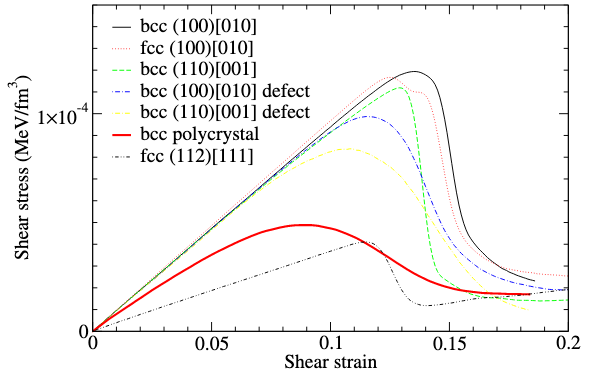
\includegraphics[width=0.6\textwidth]{pics/intro/plastic.png}
  \caption[Relation between shear stress and strain of materials in the neutron star crust]{Relation between shear stress and strain of materials in the neutron star crust for different crystal structure from the molecular dynamics simulations by \citet{2009PhRvL.102s1102H}.
  Plastic failures are triggered and release the shear stress when strain is above $\gtrsim 0.1$.}
  \label{fig:plastic-md}
\end{figure}
%

When the plastic flow is triggered, plasma viscosity will reduce the magnetic stress as well as dissipate magnetic to heat.
In response, the heated crustal material will be softened with $s_{\rm cr}$ reduced \citep{2010MNRAS.407L..54C}.
The interplay between the thermal and mechanical effects leads to the idea of thermoplastic instabilities \citep{2014ApJ...794L..24B}.
Thermoplastic waves are launched when heat released from a seed failure site diffuses to the neighboring materials and soften its critical stress below the existing shear magnetic stress.
A front of plastic failures therefore propagate in the crust, resembling the deflagration front.
The wave front propagates at the $v\sim (\chi B^2/4\pi\eta)^{1/2}$, where $\chi \sim 10$cm$^2$/s is the heat diffusion coefficient and $\eta$ is the viscosity.
Figure~\ref{fig:tpw} show the structure of the thermoplastic wave front, with $b$ being the scale magnetic, $U_{\rm th}$ being the thermal energy and $\mu_B=B^2/4\pi$.
%
\begin{figure}[h]
  \centering
  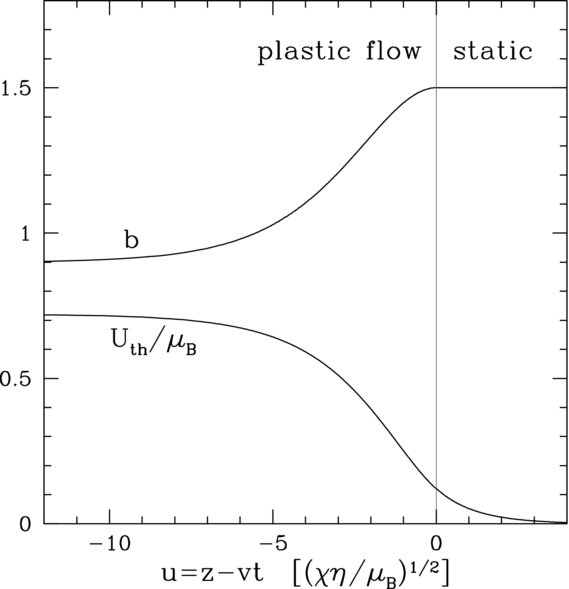
\includegraphics[width=0.6\textwidth]{pics/intro/tpw.jpg}
  \caption[Structure of the thermoplastic wave front]{structure of the thermoplastic wave front \citep{2014ApJ...794L..24B}.
  $b$ being the scale magnetic, $U_{\rm th}$ being the thermal energy and $\mu_B=B^2/4\pi$.}
  \label{fig:tpw}
\end{figure}
%

\subsubsection{Transient events}
The hard X-ray produced during giant flares and bursts must be produced outside the magnetars. 
Therefore magnetic energy must be ejected from the interior of the star to power the emission.
In the original proposal by \citet{1995MNRAS.275..255T,1996ApJ...473..322T}, magnetic energy is ejected from the interior into the magnetosphere in the form of \alfven waves.
The triggering mechanism could be the MHD instability in the liquid core or a sudden failure of the solid crust at the core-crust interface due to the build up of magnetic stress \citep{1995MNRAS.275..255T,2001ApJ...561..980T}.
Excitation of core motions with displacement $\xi$ will release energy up to $\sim E_{\rm mag}(\xi/R)^2$ where $E_{\rm mag}\sim 10^{48}$~erg is the magnetic energy in the core and $R$ is the radius of the magnetar.
The magnetic energy carried by \alfven waves are fast dissipated through turbulent cascade or magnetic reconnection.
An alternative mechanism that can trigger the release of magnetic energy into the magnetosphere is through a gradual deformation of the magnetosphere followed by a sudden of the free magnetic energy built up in the magnetosphere \citep{2003MNRAS.346..540L,2010MNRAS.407.1926G, 2013ApJ...774...92P}.
The twist of magnetosphere can be a result of crustal motions, especially plastic failures that occurs in the crust.
Strongly deformed magnetospheres can undergo global instabilities \citep{2002ApJ...572..432U}.
Numerical simulations by \citep{2013ApJ...774...92P} have demonstrated that the magnetosphere becomes unstable once the twist angle exceeds a critical value.
The free magnetic energy is released suddenly to power a flare.
This process also involves the formation of a current at the equator of the magnetosphere as shown in Figure~\ref{fig:overtwisted-magnetar}.
The current is tearing unstable and magnetic reconnection takes place which fast dissipates the magnetic energy and ejects plasmoids.
%
\begin{figure}[h]
  \centering
  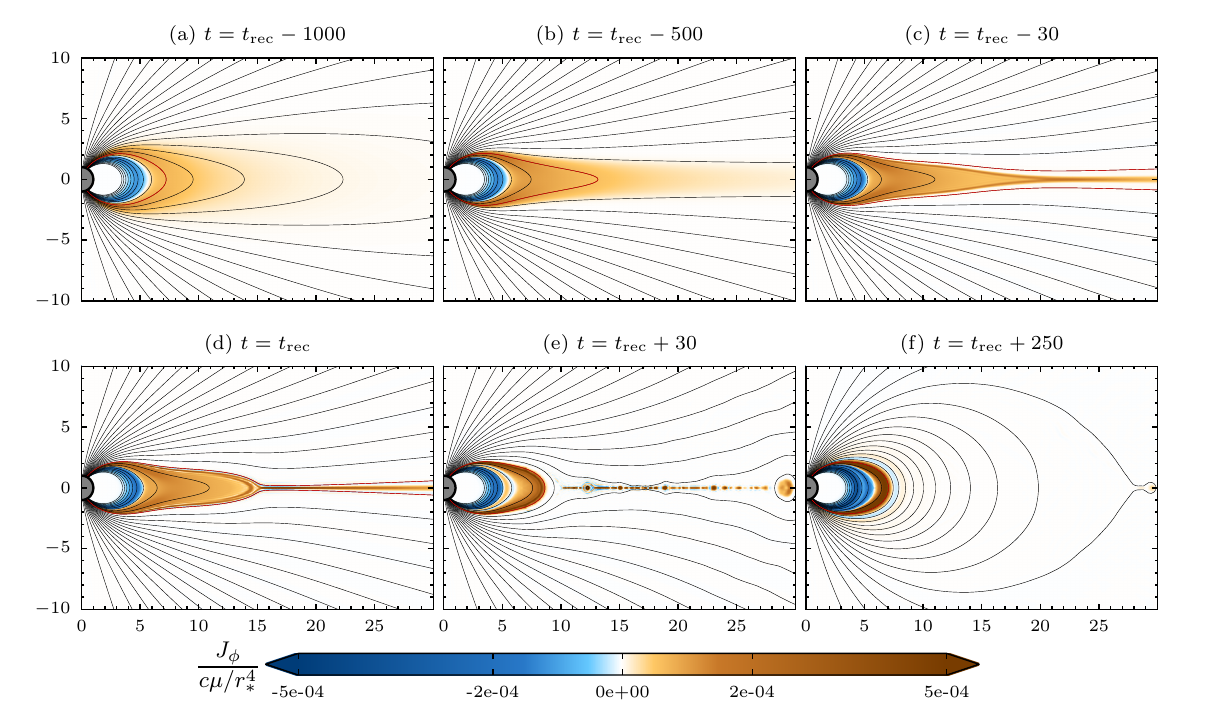
\includegraphics[width=\textwidth]{pics/intro/ffe-giant-flare.png}
  \caption[Formation of the equatorial current sheet in an over-twisted magnetar
    magnetosphere.]{Formation of the equatorial current sheet in over twisted magnetar
    magnetosphere. Color shows toroidal current density. Time is indicated in
    units of light crossing time of the star. \citep{2013ApJ...774...92P}}
  \label{fig:overtwisted-magnetar}
\end{figure}
%
The energy released during the initial spikes of giant flares are immediately thermalized, creating a fireball consisting of optically thick $e^\pm$ pair plasmas.
The evaporation of such pair plasma fireball produces the pulsating tail of the flare  \citep{1995MNRAS.275..255T,1996ApJ...473..322T}.
Besides, \alfven waves are also generated during the reconnection process.
Theses waves are trapped on the closed fields and dissipate either through nonlinear interactions \citep{1998PhRvD..57.3219T} or inside the magnetar \citep{2015ApJ...815...25L}.

\citet{2002ApJ...580L..69L} modeled the afterglow of the 1998 giant flare SGR 1900+14 by a sudden heating event in the crust.
In order to fit the observations, enormous amount of heat per unit mass is required in the outermost layer of the crust. 
How magnetic energy can heat the crust the crust to such a high level is still unclear. However, this phenomenological model has been applied to several transient magnetars to reproduce the observed light curve \citep{2013ApJ...770...65R,2014ApJ...786...62S}.

Less energetic magnetar outbursts are also considered to be trigger by the crustal motions.
Following the original ideas of \citet{1996ApJ...473..322T}, \citet{2011ApJ...727L..51P} argued that the outbursts are powered by localized releases of elastic energy in the crust  due to mechanical failures in the crystal lattice (the ``starquakes"). 
They modeled the build up of the elastic energy before each release as a result of the changing magnetic stresses, and have produced a phenomenological numerical model for the frequency of the outbursts and the magnitude of their energy release.  \citet{2012ApJ...750L...6P} have modeled the outbursts by computing the thermal flux emerging from the neutron star surface from an impulsive energy release in the crust. 


\subsubsection{Gradual untwisting of the magnetosphere}

Apart from releasing magnetic energy within a very short period of time, a twisted magnetosphere can also produce more persistent X-ray emissions through a gradual untwisting process \citep{2002ApJ...574..332T, 2009ApJ...703.1044B}.
\citet{2009ApJ...703.1044B} studied the dynamics of the twisted magnetosphere.
The nonzero $\nabla\times \boldsymbol{B}$ implies the existence of current in the magnetosphere, and the Ohmic dissipation will slowly untwist the magnetosphere.
Parallel electrical fields exist along the direction of $\boldsymbol{B}$ and lead to a longitudinal discharge voltage $\Phi_{\parallel}\sim 10^{10}$~V.
When $\Phi_{\parallel}$ is larger than a threshold value, creation of electron-positron pairs will occur and screen the parallel electrical field and therefore regulate the discharge voltage \citep{2007ApJ...657..967B}.
The main channel for pair production is through the resonant scattering of background photons.
Soft X-ray photons of a few keV from the thermal radiation of magnetars will be boosted by the electron Lorentz factor of $\gamma$ in the rest frame of electrons.
Electrons can then absorb and re-emit the photon if resonant conditions are satisfied, and the re-emitted photons have an energy boost $\sim \gamma^2$ which will produce more pairs in the magnetic field.
This process was demonstrated by the Particle-In-Cell (PIC) simulation by \citet{2017ApJ...844..133C}.

The untwisting of the magnetosphere proceeds in the following manner.
In the inner magnetosphere, a cavity with $\boldsymbol{j}=0$ is first developed which then expands and remove the current in the ``j-buldle'', the current carried by the twisted magnetosphere.
The footpoints of the j-bundle is considered to be hotter than the rest part of the magnetar surface since relativistic particles produced by the electron-positron discharge can bombard the footpoints.
As the j-bundle shrinks, the hotspot area $A$ should also shrink as well as the luminosity $L$ which gives rise to observational signatures.
Theoretical relation between $A$ and $L$ is given by$L\sim 1.33\times 10^{13} K A_{11}^2$~erg/s where $K = B_{14}\Phi_{\parallel 9}\psi$ where $\psi$ is the twisting angle.
Figure~\ref{fig:hot-spot} shows the evolution of hotspots observed for seven transient magnetars following their outbursts.
All the data points agree reasonably well with the theoretical $A-L$ relation.
%
\begin{figure}[h]
  \centering
  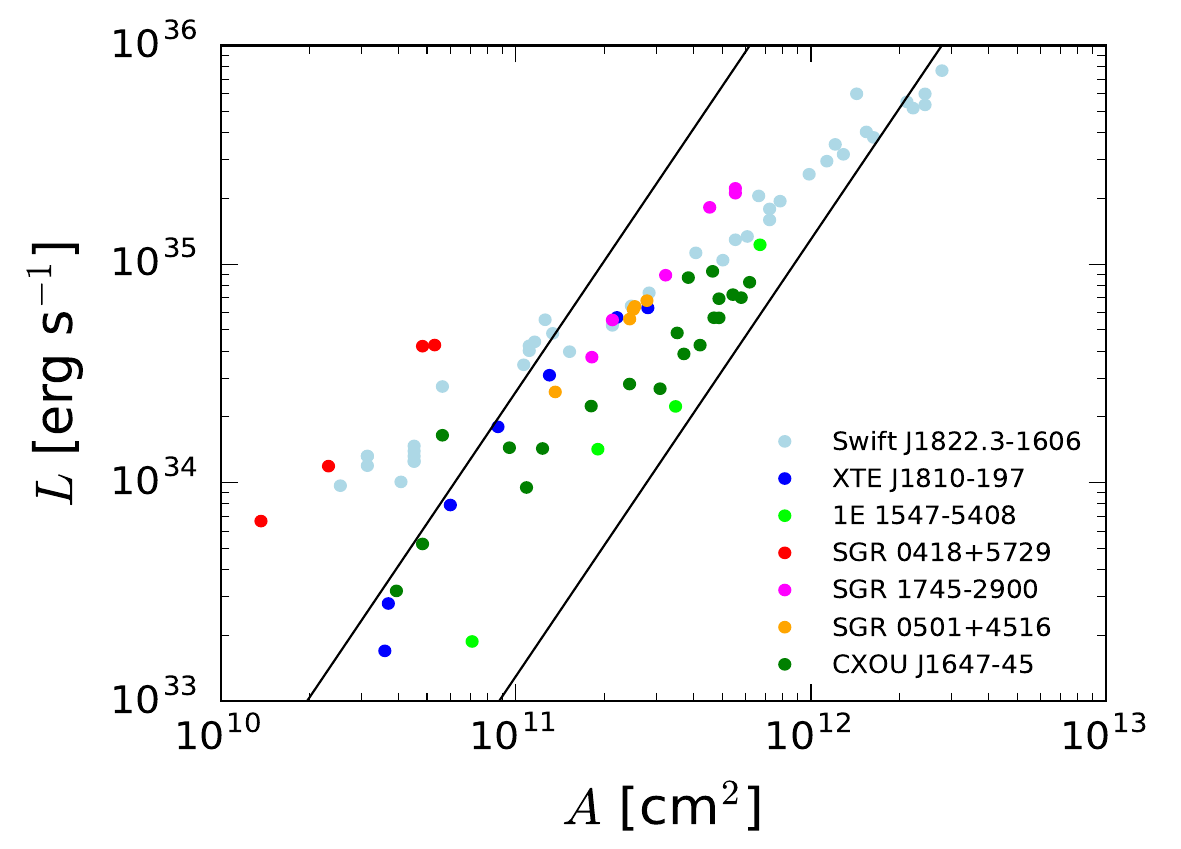
\includegraphics[width=0.6\textwidth]{pics/intro/hot-spot.png}
  \caption[The evolution of hotspots observed on transient magnetars following their outbursts]{The evolution of hotspots observed on transient magnetars following their outbursts. 
The theoretical prediction is shown by the strip between the two lines, 
$L \sim 1.3 \times 10^{33} K\,A_{11}^2$~erg~s$^{-1}$, where $K=B_{14} \Phi_9 \psi$.
The strip shown in the figure corresponds to $1<K<20$. Data for SGR 1745-2900 are 
from \citet{2015MNRAS.449.2685C};
CXOU J1647-45 from \citet{2011ApJ...726...37W} and \citet{2013ApJ...763...82A};
Swift J1822.3-1606 from \citet{2012ApJ...754...27R};
SGR 0418+5729 from \citet{2010MNRAS.405.1787E};
SGR 0501+4516 from \citet{2009MNRAS.396.2419R};
XTE J1810-197 from \citet{2007Ap&SS.308...79G};
1E 1547-5408 from \citet{2008ApJ...676.1178H} and \citet{2010PASJ...62..475E}.
The distance to 1E~1547-5408 was changed to 4~kpc following  
\citet{2010ApJ...710..227T} and \citet{2007ApJ...667.1111G}.
}
  \label{fig:hot-spot}
\end{figure}
%

Hard X-ray emissions are also produced through the resonant scattering process \citep{2013ApJ...762...13B}.
This process is sketched in Figure~\ref{fig:magnetar-loop}.
In the high magnetic field region $B>10^{13}$~G, upscattered photons are converted electron-pairs with $\gamma\approx 100(B/B_{\rm QED}$ where $B_{\rm QED}=4.4\times 10^{13}$~G.
The electron-positrons pairs form an outflow which is influenced by the radiative loss through the resonant scattering.
When the outflow of pairs reaches the region with low magnetic fields $B<10^{13}$~G, they have $\gamma\sim 1$, and upscattered photons are then able to escape leading to the hard X-ray radiation observed.
This picture provides good fit for the phase-resolved hard X-ray spectra of several magnetars \citep{2014ApJ...786L...1H,2014ApJ...789...75V,2015ApJ...807...93A}.
%
\begin{figure}[h]
  \centering
  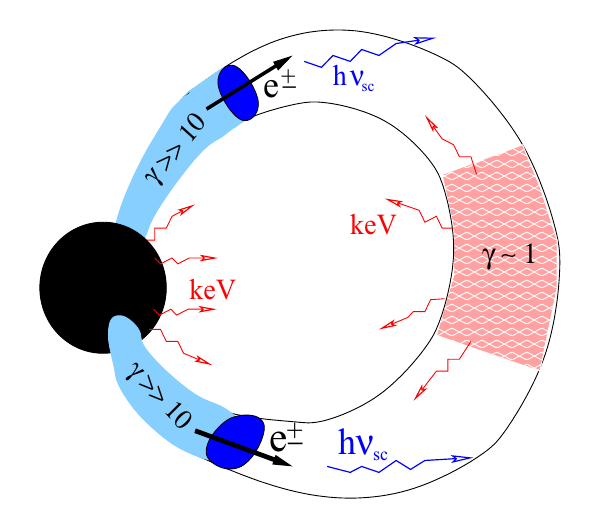
\includegraphics[width=0.5\textwidth]{pics/intro/magnetar-loop.png}
  \caption[Sketch of a twist magnetic loop.]{Sketch of a twist magnetic loop.
    Particles are accelerated in the blue region and resonantly scatter photons
    reflected from the pink region. The upscattered photons convert to pairs
    near the star, but can escape in the white region to form the observed X-ray
    spectrum \citep{2013ApJ...762...13B}.}
  \label{fig:magnetar-loop}
\end{figure}
%

\subsubsection{Magnetar heating}

The surface luminosity $10^{35}$~erg/s corresponds to the surface temperature of $T_s\approx 4\times 10^6$~K for a magnetar of radius $10-13$~km.
Typical neutron stars relax to a steady state temperature profile with constant heat flux on the conduction time $1-10$~yr after their birth.
The steady state temperature profile is isothermal at $T_{\rm core}$ in the core and most part of the crust with the temperature dropping smoothly to $T_s$ only in the outermost ``blanket'' layer $\rho<10^9$~K.
The relation of $T_{\rm core}$ and $T_s$ was established \citep{2003ApJ...594..404P} depending on the magnetic field strength and chemical composition in the blanket.
A core temperature $T_{\rm core}\gtrsim 10^9$~K is inferred from the surface luminosity of $10^{35}$~erg/s.
It is not clear how the core can sustain such a high temperature for $1-10$~kyr since neutrino emmision due to Murca process is effective in cooling the neutron star.
Heating of the core through the ambipolar diffusion may sustain the surface luminosity of $10^{35}$~erg/s. However, it requires extremely strong magnetic fields $B>10^{16}$~G and can only last for less than $1$~kyr \citep{2016ApJ...833..261B}.

Crustal heating has also been studied to explain the high surface temperature \citep{2014MNRAS.442.3484K}.
However, mechanical and ohmic heating in the crust are both limited.
Mechanical heating can only take place in the solid phase of the crust and its rate is constrained below $\sim\mu\dot{s}$ where $\mu$ is the shear modulus and $\dot{s}$ is the strain rate of deformation.
The maximum value of mechanical heating rate still falls short of the observed thermal luminosity.
The Ohmic heating rate reads $j^2/\sigma_{\rm el}$ where the conductivity $\sigma_{\rm el}\sim 10^{22}$~s$^{-1}$ for the relevant range of temperature and density in the crust \citep{2015SSRv..191..239P} and the current can be estimated through $j\sim \nabla\times B\sim \delta B/l$ as the variation of magnetic field $\delta B$ over the length scale $l$.
In order to match the observations, strong magnetic fields $\delta B>10^{16}$~G is required to vary on $l\sim 10^{4}$~cm which is not physical in the magnetar crust \citep{2016ApJ...833..261B}.

\section{This Dissertation}
\label{sec:intro-outline}

In this dissertation we will attempt to study some problems involving the dynamics of magnetic fields from the interior to the exterior of magnetars trying to answer the problem of how magnetar activities can be triggered in the crust and how magnetic energy can be dissipated to power radiations.

Chapter \ref{chap:mhd} will be a brief review of magnetohydrodynamics, its approximation in the magnetic dominated plasma -- Force-Free Electrodynamics as well as non-ideal corrections to magnetohydrodynamics.

Chapter \ref{chap:hall} will be devoted to the Hall evolution in the magnetar crust coupled with the mechanical response of the crustal material. We will propose a model for magnetar outbursts as a result of plastic crustal failures triggered by thermoplastic waves and Hall-mediated avalanches in the crust.

Chapter \ref{chap:plastic-damping} will study the interplay of magnetic evolution and crustal failures in a different setting. We will explore the fate of \alfven waves penetrating into the magnetar crust. The \alfven waves can dissipate their magnetic through triggering plastic failures which heat up the crust and power the afterglow.

Chapter \ref{chap:magnetosphere-dissipation} will focus on a competing process of \alfven wave dissipation in the magnetosphere, the turbulent cascade through the nonlinear interaction between waves. Compared with the dissipation inside the magnetar crust, turbulent dissipation is found to be slow unless the wave amplitude is much larger than the background magnetic field.

The work presented in this dissertation can be found in the following publications:
\begin{itemize}
	
\item \textit{Magnetar Outbursts from Avalanches of Hall Waves and Crustal Failures} 

Xinyu Li,  Yuri Levin and Andrei M. Beloborodov, The Astrophysical Journal, 189, 12, (2016), arXiv: 1606.04895

\item \textit{Plastic Damping of \alfven Waves in Magnetar Flares and Delayed Afterglow Emission}
 
Xinyu Li and Andrei Beloborodov, The Astrophysical Journal, 815, 25, (2015), arXiv: 1505.03465

\item \textit{Dissipation of \alfven Waves in Relativistic Magnetospheres of Magnetars}
 
Xinyu Li, Jonathan Zrake and Andrei Beloborodov, submitted to The Astrophysical Journal, arXiv: 1810.10493

\item \textit{Magnetar Heating}

Andrei Beloborodov and Xinyu Li, The Astrophysical Journal, 261, 20, (2016), arXiv: 1605.09077

\end{itemize}





% Local Variables:
% TeX-master: "../thesis"
% zotero-collection: #("16" 0 2 (name "Thesis"))
% End:
